


% Define colors for figure
%% See: http://colorbrewer2.org/
\definecolor{DEM}{HTML}{2259B3}
\definecolor{REP}{HTML}{C42B00}

\begin{figure}
  \caption{Stylized Partisan Inflation Forecast Error Predictions}
  \label{ExpectGraphs}
  \begin{center}

    \vspace{0.25cm}

    \tikzstyle{bagMain} = [text width = 5cm]
    \tikzstyle{bagDem} = [text = DEM]
    \tikzstyle{bagRep} = [text = REP]
    
    \tikzstyle{DemLine} = [draw, 
                          color=DEM,
                          opacity=0.9,
                          line width=1.5mm]

    \tikzstyle{RepLine} = [draw, 
                          color=REP,
                          opacity=0.9,
                          line width=1.5mm]

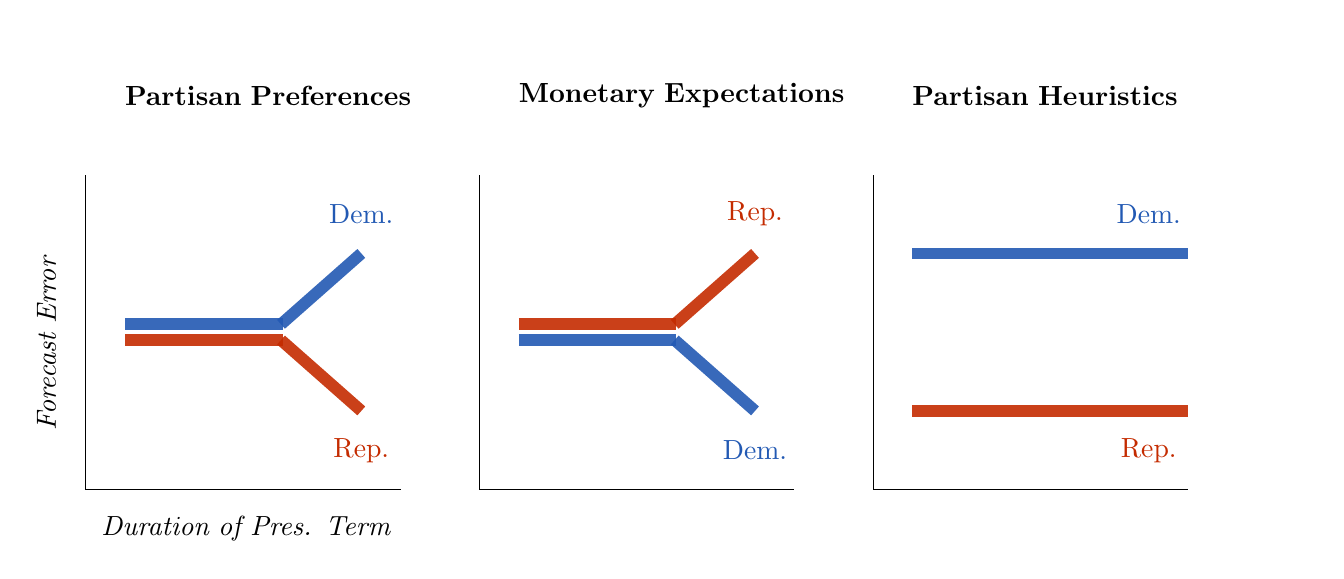
\begin{tikzpicture}

  %%%% Partisan Preferences
  \node (PP) at (-7, 5) [bagMain]{{\bf{Partisan Preferences}}};
  \node (E) at (-10.5, 3.25) [bagMain, rotate=90]{{\emph{Forecast Error}}};
  \node (T) at (-7.3, -0.5) [bagMain]{{\emph{Duration of Pres. Term}}};
  
  \draw (-10, 0) -- (-6, 0);
  \draw (-10, 0) -- (-10, 4);
  
  \draw[RepLine] (-9.5, 1.9) -- (-7.5, 1.9); 
  \draw[DemLine] (-9.5, 2.1) -- (-7.5, 2.1); 

  \draw[RepLine] (-7.52, 1.9) -- (-6.5, 1); 
  \draw[DemLine] (-7.52, 2.1) -- (-6.5, 3); 

  \node (R1) at (-6.5, 0.5) [bagRep]{Rep.};
  \node (D1) at (-6.5, 3.5) [bagDem]{Dem.};

  
  %%%% Monetary Expectations
  \node (PP) at (-2, 5) [bagMain]{{\bf{Monetary Expectations}}};
  
  \draw (-5, 0) -- (-1, 0);
  \draw (-5, 0) -- (-5, 4);
  
  \draw[RepLine] (-4.5, 2.1) -- (-2.5, 2.1); 
  \draw[DemLine] (-4.5, 1.9) -- (-2.5, 1.9); 

  \draw[DemLine] (-2.52, 1.9) -- (-1.5, 1); 
  \draw[RepLine] (-2.52, 2.1) -- (-1.5, 3); 

  \node (D2) at (-1.5, 0.5) [bagDem]{Dem.};
  \node (R2) at (-1.5, 3.5) [bagRep]{Rep.};
  
  
  %%%% Partisan Heuristics
  
  \node (PP) at (3, 5) [bagMain]{{\bf{Partisan Heuristics}}};
  
  \draw (0, 0) -- (4, 0);
  \draw (0, 0) -- (0, 4);
  
  \draw[DemLine] (0.5, 3) -- (4, 3); 
  \draw[RepLine] (0.5, 1) -- (4, 1); 

  \node (D3) at (3.5, 3.5) [bagDem]{Dem.};
  \node (R3) at (3.5, 0.5) [bagRep]{Rep.};

  \end{tikzpicture}
  \end{center}
\end{figure}


